Considérons le dessin suivant, où les mesures des angles sont en radians.

\begin{center}
	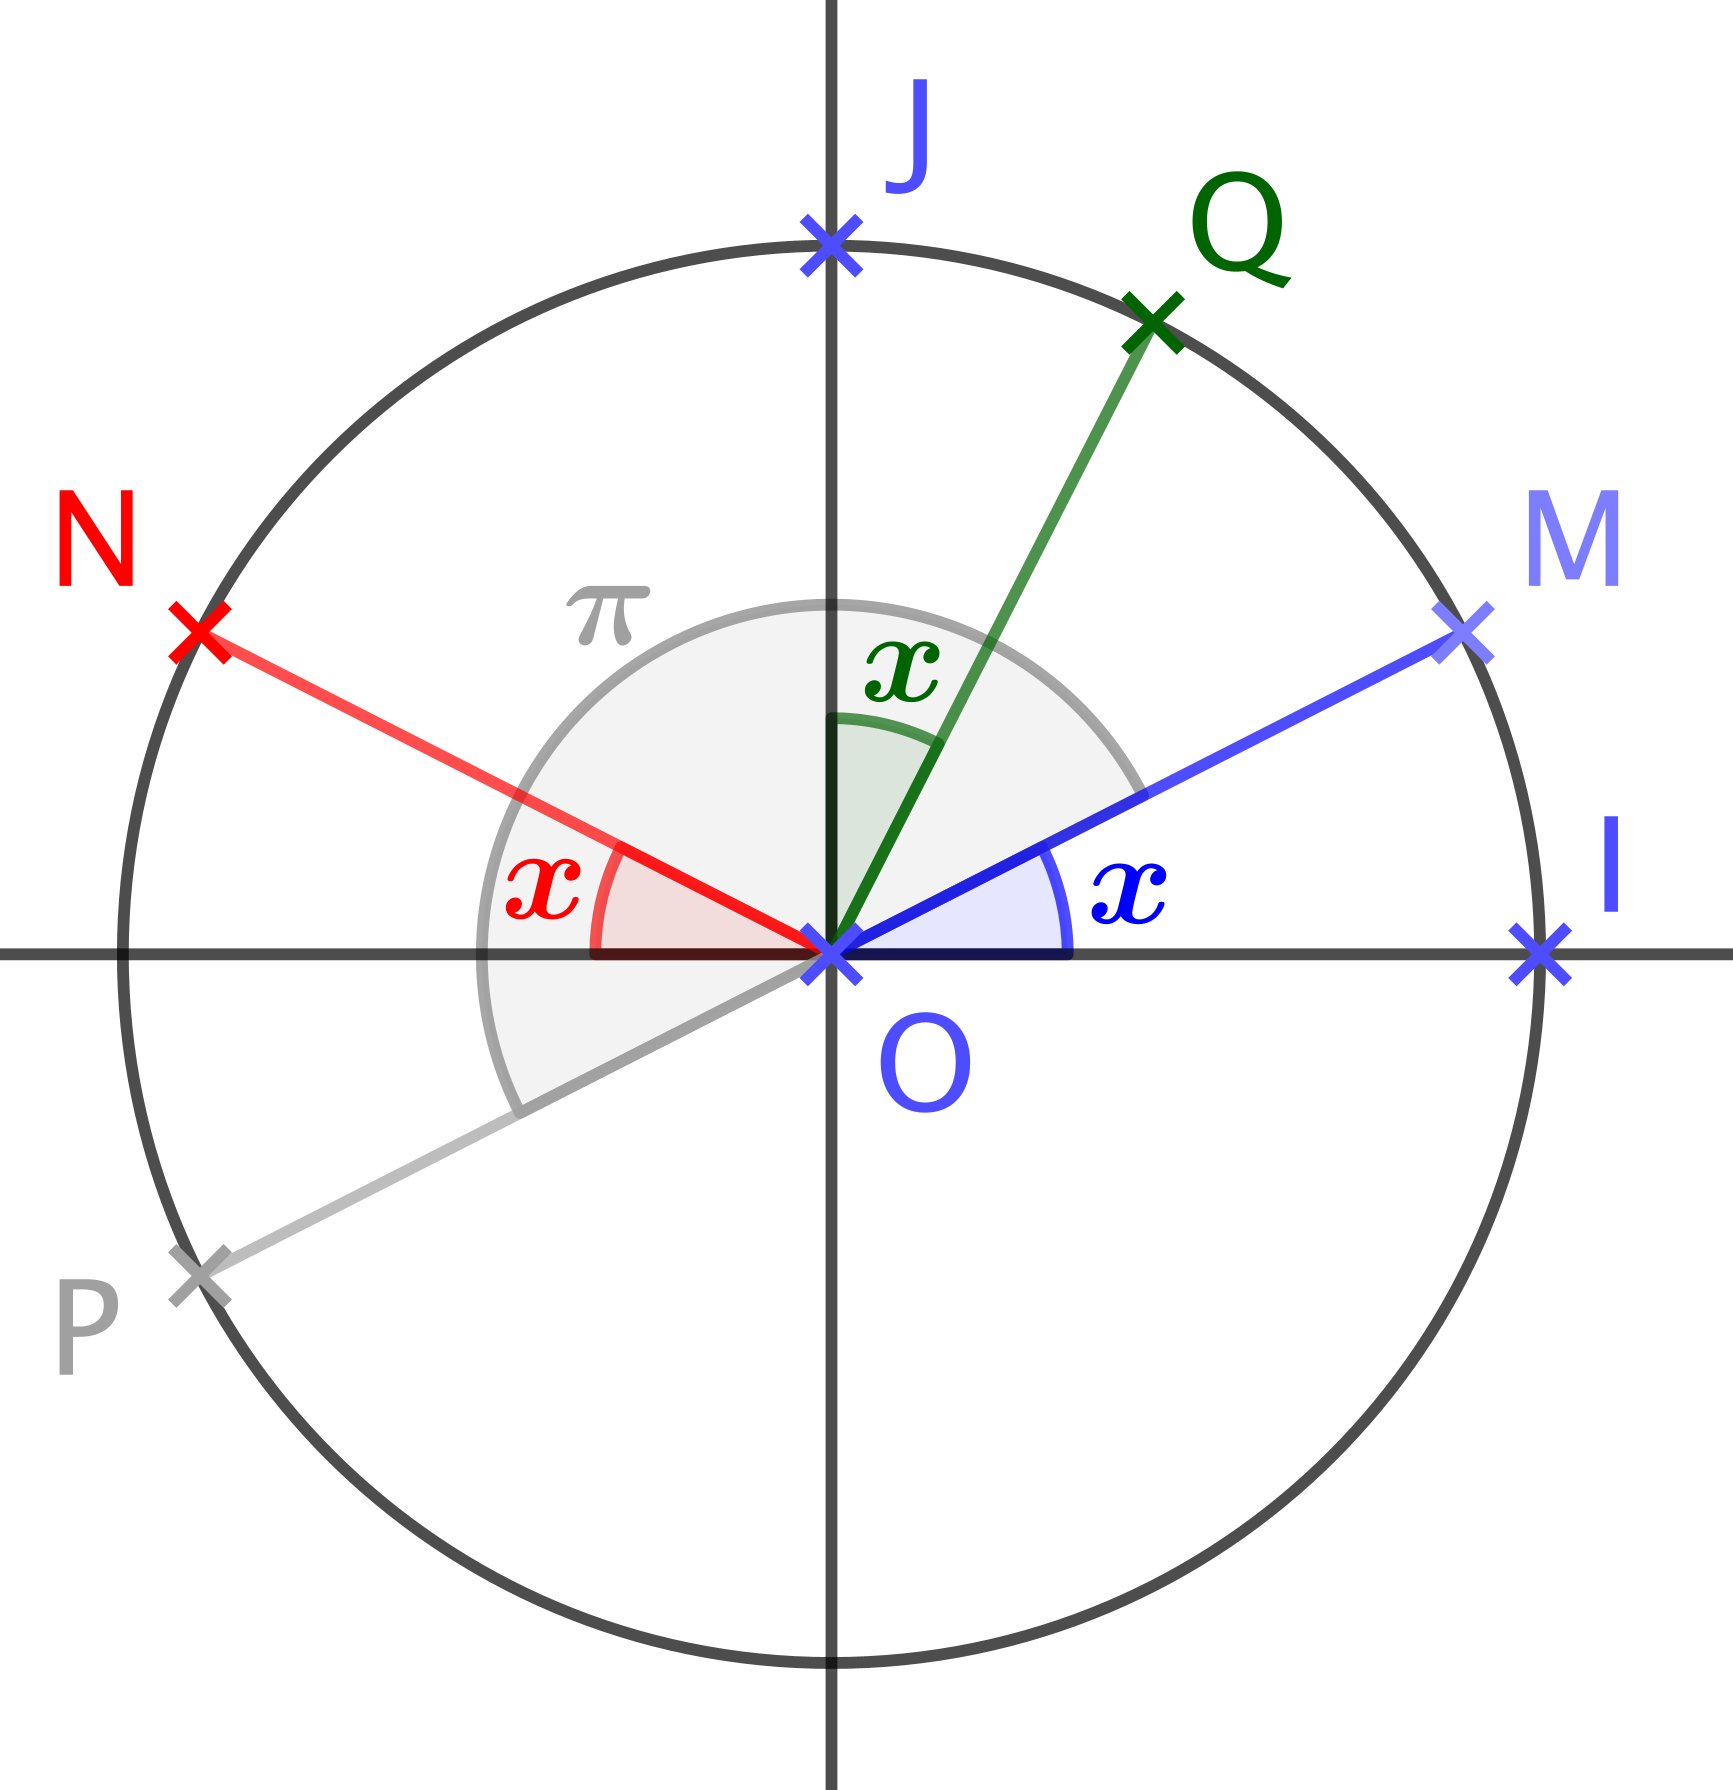
\includegraphics[scale = .7]{one-var-trig-formulas.png}
\end{center}

Via les points $M$, $N$, $P$ et $Q$, il est facile de fournir des arguments géométriques de symétrie justifiant que, sous la condition $x \in \intervalO{0}{\frac{\pi}{4}}$, nous avons:
%
\begin{multicols}{3}
\begin{itemize}[label=\small\textbullet]
	\item $\cos (\pi - x) = - \cos x$

	      \noindent
	      $\sin (\pi - x) = \sin x$ 

	\item $\cos (x + \pi) = - \cos x$

	      \noindent
	      $\sin (x + \pi) = - \sin x$

	\item $\cos \left( \frac{\pi}{2} - x \right) = \sin x$

	      \noindent
	      $\sin \left( \frac{\pi}{2} - x \right) = \cos x$ 
\end{itemize}
\end{multicols}


De nouveau, il serait bien de pouvoir passer, sans plus d'effort, à la validité des formules ci-dessus sur $\RR$ tout entier \emph{(considérer les autres cas n'est pas compliqué, mais c'est pénible)}.
%
Nous allons voir que cela est licite grâce au fait \ref{analytic-nullity} suivant qui est un peu technique, car il nécessite la notion de fonction analytique, un concept dont nous donnons la définition ci-après.


\begin{defi}
    Soit $U \subseteq \RR$ un ouvert non vide.
	Une fonction réelle $f: U \rightarrow \RR$ est dite analytique en $x_0$, 
	s'il existe
	une série entière $\dsum_{n \geq 0} a_n x^n$
	de rayon de convergence $\rho_0 > 0$,
	et
	un réel $r \in \intervalOC{0}{\rho_0}$ tels que 
	$\forall x \in \intervalO{x_0 - r}{x_0 + r} \subseteq U$, on ait:
	$f(x) = \dsum_{n \geq 0} a_n (x - x_0)^n$.
	%
	Si $f$ est analytique en tout réel de $U$, on dira que $f$ est analytique sur $U$.
\end{defi}



\begin{fact} \label{analytic-nullity}
    Soit $U \subseteq \RR$ un ouvert connexe non vide,
    et
    $f: U \rightarrow \RR$ une fonction analytique non identiquement nulle.
    %
	Si $\alpha \in U$ vérifie $f(\alpha) = 0$,
	alors il existe un ouvert $V$ tel que 
	$\alpha \in V \subseteq U$,
	et
	$\forall x \in V - \setgene{\alpha}$, $f(x) \neq 0$ 
	\emph{(c'est le principe des zéros isolés)}. 
\end{fact}


\begin{proof}
	TODO
\end{proof}








\newpage

Si nous revenons à nos identités trigonométriques, il suffit de savoir que les fonctions circulaires réelles sont analytiques sur $\RR$ tout entier, et de noter que le raisonnement géométrique au début de cette section fait clairement apparaître des zéros non isolés pour les fonctions analytiques sur $\RR$ suivantes.%
\footnote{
	Nous admettrons ces affirmations qui ne sont pas violentes à démontrer une fois que l'on a les bases de la théorie des fonctions analytiques.
}
%
\begin{itemize}[label=\small\textbullet]
	\item $f_1(z) = \cos (\pi - z) + \cos z$ 
	   et $f_2(z) = \sin (\pi - z) - \sin z$ 

	\smallskip
	\item $f_3(z) =\cos (z + \pi) + \cos z$ 
	   et $f_4(z) =\sin (z + \pi) + \sin z$

	\smallskip
	\item $f_5(z) =\cos \left( \frac{\pi}{2} - z \right) - \sin z$ 
	   et $f_6(z) =\sin \left( \frac{\pi}{2} - z \right) - \cos z$ 
\end{itemize}


Que faire si nous avons des formules trigonométriques impliquant deux variables? Par exemple, le dessin suivant, par simple application des définitions géométriques du cosinus et du sinus, donne à la fois
$\cos(\alpha + \beta) = \cos \alpha \cos \beta - \sin \alpha \sin \beta$
et
$\sin(\alpha + \beta) = \cos \alpha \sin \beta + \sin \alpha \cos \beta$
pour
$(\alpha ; \beta) \in \big( \RRsp \big)^2$ tel que $0 < \alpha + \beta < \frac{\pi}{2}$. 

\begin{center}
	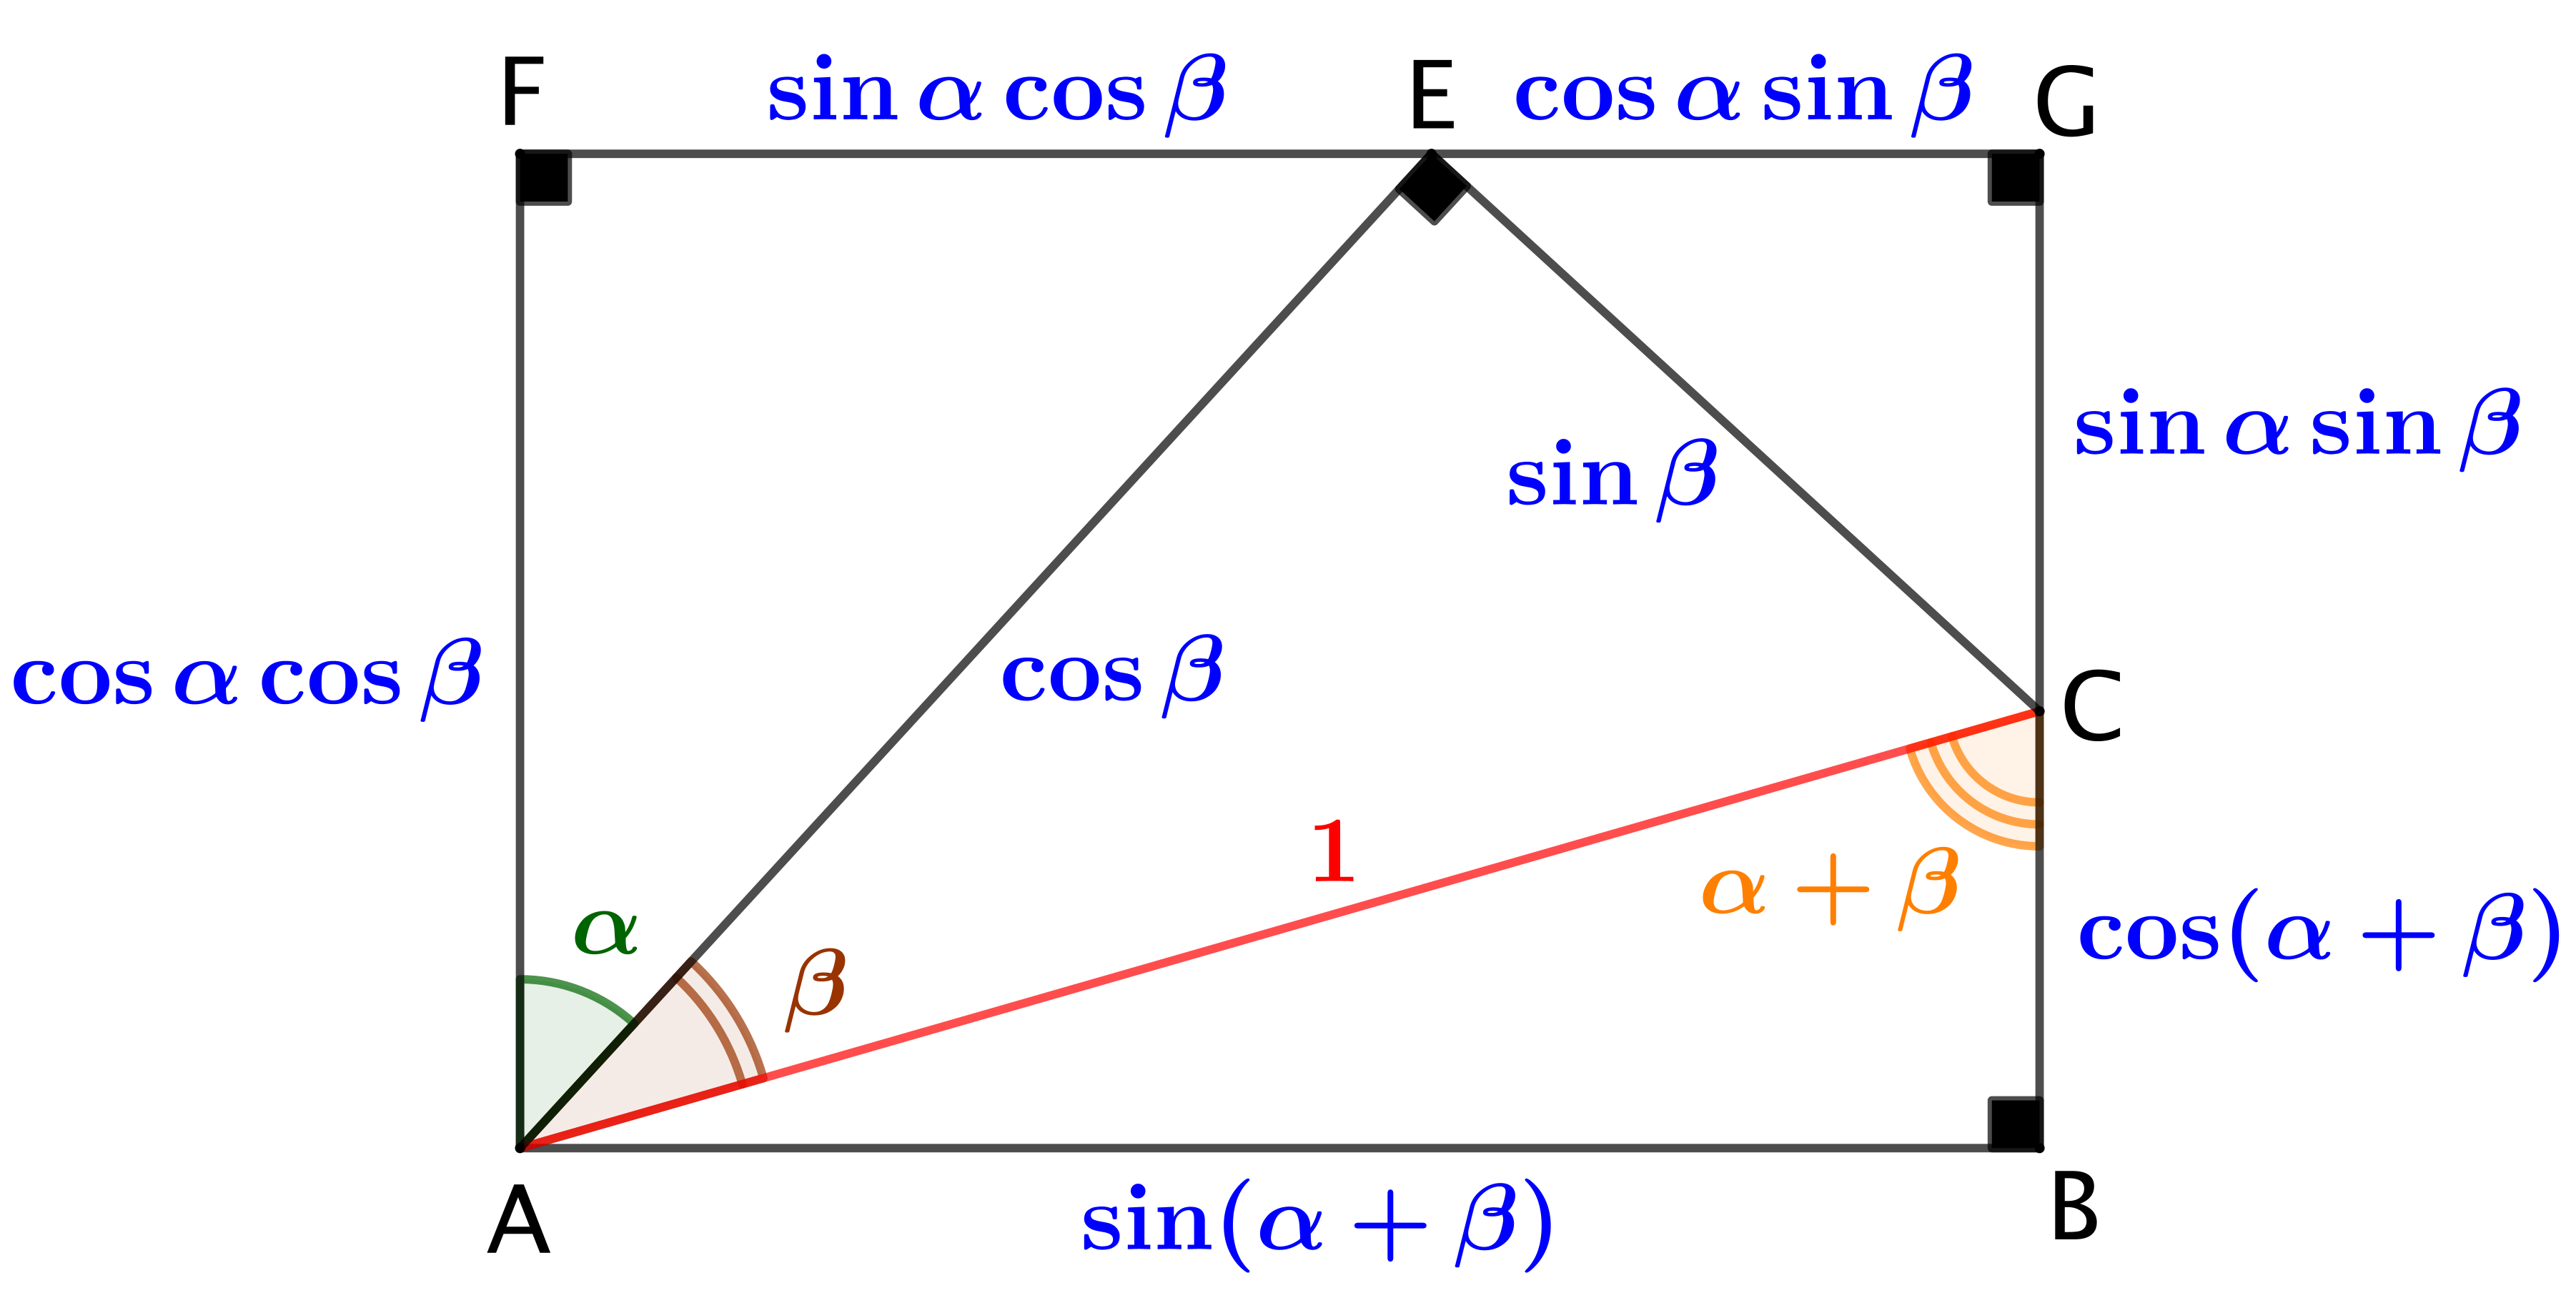
\includegraphics[scale=.7]{two-var-trig-formulas.png}
\end{center}

Le fait \ref{multi-analytic-nullity} ci-dessous, qui généralise le fait \ref{analytic-nullity}, implique la validité des formules trigonométriques précédentes sur $\RR^2$ tout entier en faisant les choix ci-après.
Nous voilà sauvés!
%
\begin{itemize}[label=\small\textbullet]
	\item $f_1(\alpha ; \beta) = \cos(\alpha + \beta) - \cos \alpha \cos \beta + \sin \alpha \sin \beta$

	\item $f_2(\alpha ; \beta) = \sin(\alpha + \beta) - \cos \alpha \sin \beta - \sin \alpha \cos \beta$
\end{itemize}


\begin{defi}
    Soient $n \in \NNs$, et $\Omega \subseteq \RR^n$ un ouvert non vide.
	Une fonction complexe $f: \Omega \rightarrow \RR$ est dite analytique en $\omega \in \Omega$, 
	si elle est $\RR$-différentiable en $\omega$,
	c'est-à-dire s'il existe une application $\RR$-linéaire $Df: \RR^n \rightarrow \RR$
	vérifiant
	$\displaystyle \lim_{\stackrel{\norm{z - \omega}_n \, \rightarrow \, 0}{z \, \in \, \Omega - \setgene{\omega}}}\!\Big( \frac{f(z) - f(\omega) - Df(\omega) (z - \omega)}{\norm{z - \omega}_n} \Big) = 0$.
\end{defi}


\begin{fact} \label{multi-analytic-nullity}
    Soient $n \in \NN_{\geq 2}$,
    $\Omega \subseteq \RR^n$ un ouvert connexe non vide,
    et
    $f: \Omega \rightarrow \RR$ une fonction analytique.
    %
	Si $f$ s'annule sur un ouvert de $\Omega$,
	alors $f$ est identiquement nulle
	\emph{(c'est le théorème d'identité)}. 
\end{fact}


\begin{proof}
	Ceci nous amènerait trop loin, donc nous admettrons ce résultat. Si vous avez une impression de déjà-lu, c'est normal.
\end{proof}
